\documentclass{standalone}
%\documentclass[a4paper,10pt]{scrartcl}

\usepackage[utf8]{inputenc}
\usepackage{tikz}
\usetikzlibrary{fit}

\begin{document}

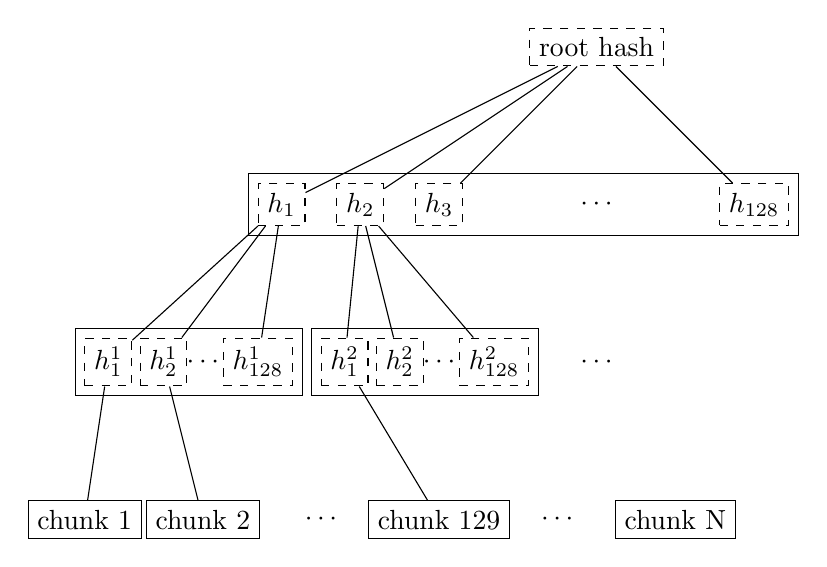
\begin{tikzpicture}
\node[draw,dashed] (root) at (5,3) {root hash};
\node[draw,dashed] (h1) at (1,1) {$h_1$};
\node[draw,dashed] (h2) at (2,1) {$h_2$};
\node[draw,dashed] (h3) at (3,1) {$h_3$};
\node (dots) at (5,1) {$\cdots$};
\node[draw,dashed] (h128) at (7,1) {$h_{128}$};
\node[draw,fit=(h1) (h2) (h3) (dots) (h128)]{};
\draw (root) -- (h1);
\draw (root) -- (h2);
\draw (root) -- (h3);
\draw (root) -- (h128);
\node[draw,dashed] (g1) at (-1.2,-1) {$h^1_1$};
\node[draw,dashed] (g2) at (-0.5,-1) {$h^1_2$};
\node (gdots) at (0,-1) {$\cdots$};
\node[draw,dashed] (g128) at (0.7,-1) {$h^1_{128}$};
\draw (h1) -- (g1);
\draw (h1) -- (g2);
\draw (h1) -- (g128);
\node[draw,fit=(g1)(g2)(gdots)(g128)]{};
\node[draw,dashed] (f1) at (1.8,-1) {$h^2_1$};
\node[draw,dashed] (f2) at (2.5,-1) {$h^2_2$};
\node (fdots) at (3,-1) {$\cdots$};
\node[draw,dashed] (f128) at (3.7,-1) {$h^2_{128}$};
\draw (h2) -- (f1);
\draw (h2) -- (f2);
\draw (h2) -- (f128);
\node[draw,fit=(f1)(f2)(fdots)(f128)]{};
\node (moredots) at (5,-1) {$\cdots$};
\node[draw] (c1) at (-1.5,-3) {chunk 1};
\node[draw] (c2) at (0,-3) {chunk 2};
\node at (1.5,-3) {$\cdots$};
\node[draw] (c129) at (3,-3) {chunk 129};
\node (cdots) at (4.5,-3) {$\cdots$};
\node[draw] (cn) at (6,-3) {chunk N};
\draw (g1) -- (c1);
\draw (g2) -- (c2);
\draw (f1) -- (c129);
\end{tikzpicture}\\
\end{document}
